%!TEX program = xelatex
\documentclass[cn,black,12pt,device=normal]{elegantnote}
\usepackage{hyperref}
\usepackage{tikz}
\usepackage{float}
\usepackage{caption}
\usepackage{subcaption}
\usepackage{amsmath}
\usepackage{amsfonts}
\usepackage{amssymb}
\usepackage{siunitx}
\usepackage{graphicx}
\usepackage{wasysym}



\usetikzlibrary{positioning, shapes.geometric}
\tikzstyle{block} = [draw,rectangle,rounded corners=3mm,text centered, text width=8em, minimum height = 15mm,minimum width = 25mm]
%\newcommand{\upcite}[1]{\textsuperscript{\textsuperscript{\cite{#1}}}}
\renewcommand{\figurename}{Fig.}
\renewcommand{\contentsname}{Contents}

\title{Lab Report\\2020-2021 Spring Term}

\author{姜文渊\\ID: 1951510}
\institute{School of Life Science, Tongji University}

\date{\today}

\usepackage{array}

\begin{document}

\maketitle
\tableofcontents
\newpage

\newpage
\section{Report 01: Overview of the project}

\subsection*{2021-03-04}

\subsection{Introduction}
The project of this semester involves the application of our \textit{Drosophila melanogaster} model
on some environment issues. 

Persistent organic pollutants (POPs) are toxic chemicals 
that adversely affect human health and the environment around the world. 
Studies have linked POPs exposures to declines, 
diseases, or abnormalities in a number of wildlife species, including certain kinds of fish, birds, and mammals. 
In people, reproductive, developmental, behavioral, neurologic, endocrine, 
and immunologic adverse health effects have been linked to POPs.\cite{ashraf2017persistent}

Evidence has shown that cancer is linked with POPs exposures\cite{hardell2006utero}, but little is known about
the impact of \textbf{Persistent Organic Pollutants (POPs)} on \textbf{tumor migration}, 
which plays a key role in the occurrence of cancer.

In the first session of this course, 
we discussed how to investigate the impact of Persistent Organic Pollutants (POPs) on tumor migration,
with our \textit{Drosophila melanogaster} model.
We have made a brief design of the experiments of this semester and chosen several POPs to study, 
using \textit{Drosophila melanogaster} with activated $Ras^{v12/Ig}$ gene and $eyeful$ \textit{Drosophila}.
We also planned to investigate which of the pathways are involved in the tumor migration
caused by POPs and we wanted to explore the mechanism behind the migration, if possible.

\subsection{Experiment design}
The main idea of our experiments is to construct some \textit{Drosophila} models for the study of tumor migration 
and then expose our \textit{Drosophila} models to different levels of certain POPs to observe the outcomes.

Traditional methods in genetics and molecular biology will be utilized, including the Fluorescence microscopy,
Quantitave reverse transcription polymerase chain reaction,
Western blot, and etc.
Some analytical techniques which are not common in the field of biology may also be used, 
such as the High-performance liquid chromatography (HPLC) and the High-performance gas chromatography (HPGC).

\subsection{Plan for this semester}
The following experiments is planned to do in this semester:
\begin{itemize}
    \item Selection and construct of \textit{Drosophila} models
    \item \textit{Drosophila} crossing
    \item \textit{Drosophila} stock maintaince
    \item Preparation of the POPs sample
    \item \textit{Drosophila} disection
    \item Fluorescence microscopy
    \item RT-qPCR
    %\item Western blot
    \item HPLC/GC
\end{itemize}

\subsection{Results \& Discussion}

In this section, we are introduced to a new project, which involves applying our knowledge and skills to environment issues. The background of this project and the techniques that will be used is shwon above, and more detailed record of the design and implementation of the experiments will be talked in the following reports.

\newpage
\section{Report 02: Experiment design}

\subsection*{2021-03-18}


\subsection{Introduction}
In this session, we discussed about the experiments that will be done next, with more details. 
The research route is illustrated below.
\begin{figure}[H]
    \centering
    \begin{subfigure}{.5\textwidth}
      \centering
      %\includegraphics[width=.4\linewidth]{image1}
      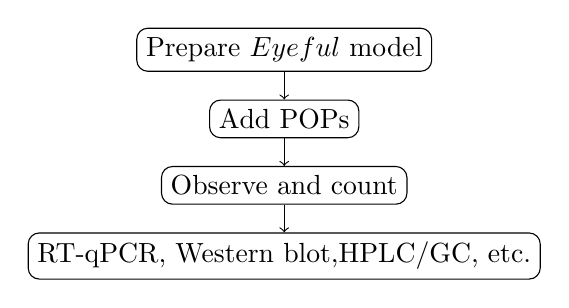
\begin{tikzpicture}[node distance=10pt]
        \node[draw, rounded corners]                (A1)  {Prepare $Eyeful$ model};
        \node[draw, rounded corners, below=of A1]   (A2)  {Add POPs};
        \node[draw, rounded corners ,below=of A2]   (A3)  {Observe and count};
        \node[draw, rounded corners ,below=of A3]   (A4)  {RT-qPCR, Western blot,HPLC/GC, etc.};
    
        \draw[->] (A1) -- (A2);
        \draw[->] (A2) -- (A3);
        \draw[->] (A3) -- (A4);
      \end{tikzpicture}
      \caption{$Eyeful$ model}
      \label{fig:sub1}
    \end{subfigure}%
    \begin{subfigure}{.5\textwidth}
      \centering
      %\includegraphics[width=.4\linewidth]{image1}
      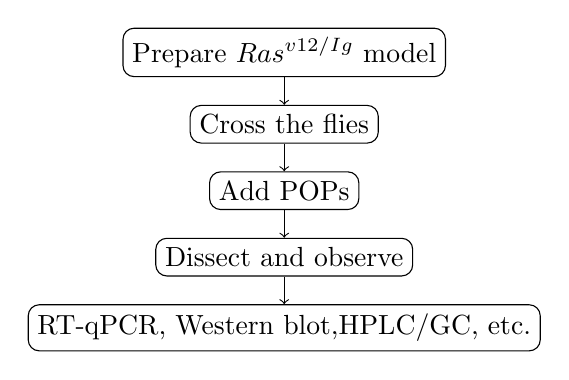
\begin{tikzpicture}[node distance=10pt]
        \node[draw, rounded corners]                (A0)  {Prepare $Ras^{v12/Ig}$ model};
        \node[draw, rounded corners, below=of A0]   (A1)  {Cross the flies};
        \node[draw, rounded corners, below=of A1]   (A2)  {Add POPs};
        \node[draw, rounded corners, below=of A2]   (A3)  {Dissect and observe};
        \node[draw, rounded corners, below=of A3]   (A4)  {RT-qPCR, Western blot,HPLC/GC, etc.};
    
        \draw[->] (A0) -- (A1);
        \draw[->] (A1) -- (A2);
        \draw[->] (A2) -- (A3);
        \draw[->] (A3) -- (A4);
      \end{tikzpicture}
      \caption{$Ras^{v12/Ig}$ model}
      \label{fig:sub2}
    \end{subfigure}
    \caption{Scheme of the experiments}
    \label{fig:test}
\end{figure}

\subsection{Our \textit{Drosophila} models}
To study the potential impact of POPs on tumor migration, we used two well established models.

\subsubsection{$Eyeful$ model}
One of the two models is the $Eyeful$ flies\cite{ferres2006epigenetic}, which will be crossed with the \textit{w1118} flies. 
Since $Eyeful$  flies have distinct phenotype that indicates whether there is a tumor migration, 
it is a desirable model for this study. 
Moreover $Eyeful$ flies can be used to study the effect of POPs on different generations.


\subsubsection{$Ras^{v12/Ig}$ model}
The other model is the $Ras^{v12/Ig}$ model. Dissection is needed in 3rd pupa,
and with GFP, this model can produce more accurate information about the migration of tumor cells.
However, this model is used by crossing two stocks, and the larva can not survive the 3rd period.

\subsection{Results \& Discussion}

In this section, we talked with the tutor about the scheme of the experiments that will be done this term. In short, \textbf{preparation of model \textit{Drosophila} will be the first part of the experiments, and the most crucial part is the POPs treatment of the models}. With properly treated models, subsequential measurement could be done, for example, the qPCR, Western bolt or even HPLC/GC, etc.

\newpage
\section{Report 03: Building model \textit{Drosophila}}

\subsection*{2021-04-01}

\subsection{Introduction}
Before carrying out the experiments, model \textit{Drosophila} should be prepared using molecular and genetic methods. In this session, we discussed about the details of constructing the model \textit{Drosophila} needed in next experiments.


\subsection{Results \& Discussion}
Since the two models are based on different mechanisms, we will talk about how these models work and how to construct them respectively.

\subsubsection{$Eyeful$ model}
The typical phenotype of $Eyeful$ are eye tumours and metastases, which is shown in the figure below.\cite{ferres2006epigenetic}
\begin{figure}[H]
    \centering
    \includegraphics[width=0.7\textwidth]{image/eyeful_phenotype.png}
    \caption{Typical phenotype of $Eyeful$, from Ferres-Marco, D., Gutierrez-Garcia, I., Vallejo, D. et al. Epigenetic silencers and Notch collaborate to promote malignant tumours by Rb silencing. Nature 439, 430–436 (2006).}
    \label{eyeful_phenotype}
\end{figure}

According to Ferres et al., the eye tumours and metastases in the $Eyeful$ model are induced by two genes: \textit{psq} and \textit{lola}, together with the overexpression of \textit{Delta}. The mechanism behind eyeful and tumor metastases is that eyeful forces the transcription of two hitherto unsuspected growth and epigenetic genes, \textit{lola} and \textit{pipsqueak (psq)}, leading to changes of epigenetic pathways in growth control and tumorigenesis.\cite{ferres2006epigenetic}

The $Eyeful$ files we used in our experiments are constructed by Ferres et al. They used the Gene Search (GS) system to find genes that induces big eye phenotype with the overexpression of \textit{Delta}, and produced the $Eyeful$ line. 

The technique used to build the $Eyeful$ model is the gene search system, reported by Toba, G. et al.\cite{toba1999gene} The scheme of the technique is shown in the figure below.

\begin{figure}[H]
    \centering
    \includegraphics[width=0.7\textwidth]{image/gene_search.png}
    \caption{Schematic representation of the gene search system; by Toba, G. et al.}
    \label{eyeful_phenotype}
\end{figure}

In short, the gene search system involves the random insertion of a vector, which contains two copies of the upstream activating sequence (UAS) enhancer adjacent
to a core promoter, one copy near the terminal inverted repeats at each end of the vector, and oriented
to direct transcription outward. 

The vector is inserted to a $ey–Gal4 > Dl$ line (a triple mutant strain carrying the eyeful, UAS–Dl and ey–Gal4 transgenes all on the same chromosome) randomly, and the out-coming phenotype are screened.

\subsubsection{$Ras^{v12/Ig}$ model}
The $Ras^{v12/Ig}$ model consists of two lines:
\begin{enumerate}
    \item w;$Igl^4$ FRT40A UAS-$RAS^{v12}$/CyO;Sb/TM6B Tb
    \item yw ey-Flp; tub-Gal80 FRT40A; act>y+>Gal4 UAS-$GFP$
\end{enumerate}
The first line is used as the line to produce tumours and metastases in eye, brain and ventral nerve cord (VNC), while the second line with Gal4 is used to trigger the tumours and metastases in the former line, when the two lines are crossed.

Note that in the second line, ey-Flp is used. Flp-FRT recombination is a site-directed recombination technology, increasingly used to manipulate an organism's DNA under controlled conditions \textit{in vivo}. Different types of Flp-FRT recombination are briefly illustrated below.

\begin{figure}[H]
    \centering
    \includegraphics[width=0.25\textwidth]{image/Flp-FRT.png}
    \caption{Different types of Flp-FRT recombination}
    \label{Flp-FRT}
\end{figure}

The last type of Flp-FRT recombination explains how our model works. In \textit{Drosophila}, homozygous 
$Igl^4$ leads to lethal before larva of the 3rd instar, and therefore should be avoided in early stages of development. When the larva enters 3rd phase, ey-Flp can be properly expressed in the eye disc, leading to Flp-FRT recombination happen randomly during mitosis. The figure below shows how Flp-FRT recombination in our model.

\begin{figure}[H]
    \centering
    \includegraphics[width=0.7\textwidth]{image/FRT_RAS.png}
    \caption{How Flp-FRT recombination in our model; by Pagliarini, Raymond A and Xu, Tian}
    \label{FRT-RAS}
\end{figure}

Expression of the FLP recombinase in the developing eye ey-FLP mediates mitotic recombination between chromosome arms and produces clones of cells homozygously mutant for a gene that promotes metastatic behavior(i.e., scrib). Only these mutant cells lose the Gal80 repressor, which allows Gal4 of the eyFLP-activated Act>y>Gal4 “flip-out” construct to direct the constitutive expression of UAS-GFP and UAS-RasV12 (as well as othergenes of interest) regardless of their eventual locations and differentiation status. Gal80 expression in nonmutant cells also markedly reduces leaky flip-out construct expression in tissues outside of the eyeantennal region. Expression of GFP, RasV12, and other transgenes is therefore restricted to homozygous mutant cells. Multiple genetic alterations can be combined in the same cell and metastatic behavior can be monitored in vivo by following these GFP-expressing cells.\cite{pagliarini2003genetic}

Microinjection of the P-element plasmid which contains our target sequence into \textit{Drosophila} eggs is a common practise of building model files, and the P-element plasmid will be integrated to the genome. The files are then screened by their eye color, and crossed with tool files. Tool files are those files with double balancer chromosomes. After the crossing, desired chromosome will be identified and will become an allele chomosome with a balancer chromosome.


\newpage
\section{Report 04: Stock maintaince}

\subsection*{2021-04-15}

\subsection{Introduction}
		
In this session, we will practise the basic skills commonly used in \textit{Drosophila} experiments. 
	
\subsection{Materials \& Methods} 
		The following protocol is modified based on \textit{Drosophila Maintenance Protocol} \cite{dros2017} according to the preference of our lab.
	\subsubsection{Nutrition} \textit{Drosophila} subsists on the microorganisms, such as yeast, that grow on fermenting fruit. In the lab, the fly’s diet is modified for practical purposes. Several recipes are available, and all contain the essential components: sugar and yeast. The following recipe is adopted in our lab. 
			\begin{enumerate}
				\item Water: \SI{1000}{\milli\liter}
				\item Brown sugar: \SI{135}{\gram}
				\item Agar: \SI{7}{\gram}
				\item Yellow cornmeal: \SI{135}{\gram}
				\item Yeast: \SI{8}{\gram}
				\item Propionic acid: \SI{1000}{\milli\liter}
			\end{enumerate}
			These ingredients are combined, heated, stirred, and then distributed into glass or plastic housing vials. After they are filled, the vials are plugged with a cotton top, wrapped, and cooled.
			
	\subsubsection{Housing} A variety of containers are used for housing \textit{Drosophila}. Vials are used in our lab for fly maintenance and optimally contain 50-100 adults, while other labs may use bottles, which can house 300-600 adult flies, for larger cultures. Incubators control the environment and are capable of holding hundreds of vials and bottles. The normal storage conditions for flies are \SI{25}{\celsius} with  60-65\% relative humidity, but for some stocks (eg. \textit{tub}-${Gal80}^{ts}$ and some special $Gal4$), a temperature of \SI{18}{\celsius} or \SI{29}{\celsius} is needed.
			
			
	\subsubsection{Handling} 
		When working with flies, it is important to practice proper labeling and documentation, and to keep a clean environment to maintain the integrity of fly lines and experiments. A container must be changed when about half of the pupae have eclosed, or left the pupal casing. The casings will appear clear.\par
			
		The pupal stage occurs between the larval and adult stages, and is the time when the larvae incubate and develop into an adult. To identify pupal casings as clear, hold the container up to a light source and inspect the pupa. \par 
			
		Flies are transferred to vials with fresh media via a process known as "flipping flies." Before flipping flies, inspect the media for integrity. Flies cannot survive on food cracked with dryness or contaminated with mold or bacteria. \par 
			
		To flip flies, first, tap the fly vial gently on the counter to knock flies off the sides of the vial. Then quickly remove the stopper, and invert the flies from the old container rapidly into a new one. This process is done rapidly, to prevent flies from escaping or being crushed by the stopper, and to prevent loose flies from entering the vial during flipping. \par 
			
			

	\subsubsection{Anesthetization} Anesthetization is required for sorting flies. Two methods of anesthetization will be discussed here: chilling, and using carbon dioxide.\par
			
		To chill flies place the culture in a \SI{-20}{\celsius} freezer for 8-12 minutes. Then place flies onto a chilled, flat workspace for selection. Flies can also be anesthetized using cold by chilling them directly on a frozen surface. \par 
			
		Carbon dioxide is a preferred method for anesthetization because it does not cause acute mortality in flies. This method is adopted in our lab. The $CO_{2}$ delivery system is made up: of a $CO_{2}$ tank; a tube connected to a needle, to anesthetize flies in vials and bottles; and a tube connected to a $CO_{2}$ plate for analysis under the microscope. \par 
			
		To anesthetize flies, insert the $CO_{2}$ needle through the stopper. Alternatively, tap the container on a surface, remove the stop, and quickly invert the flies onto a $CO_{2}$ plate, keeping a closed seal until the flies are immobile. Using a brush or forceps, gently move the flies into the new container. \par 
			
		To discard unwanted flies, dump them into a fly morgue, which consists of a large bottle filled with isopropanol or ethanol and mineral oil topped with a funnel. \par 
	
	\subsection{Results \& Discussion} 
		In this session, we used the \textit{w1118} stock for practising the skills mentioned above. Most of the operations are easy to perform except the "flipping flies", which takes time to get dexterity. 


\newpage
\section{Report 05: POPs treatment of the $Eyeful$ model (Chlordecone)}

\subsection*{2021-04-29}

\subsection{Introduction}

With the $Eyeful$ model built in last experiment, we are now able to use different kind of POPs to treat the model flies and collect relevant data about the impact of POPs on \textbf{tumor migration}.

Other phenotypes, such as the \textbf{adult survival rate}, \textbf{reproductive capacity} and \textbf{body weight} will also be measured, if possible. These data can be used to study the overall effects of POPs, and they can provide clues about the factors behind tumor migration.

\subsection{Experiment Design}

\subsubsection{POPs gradients}
The setting of the POPs gradients used in the experiments is of much importance for their implementation.
For the convenience of calculation and dilution, we choose \textbf{Mass fraction} ($m_{POPs}/m_{fly food}$) as the unit of concentration.
According to previous literature and the real situation of the POPs pollution, we choose several POPs, which are listed in the table below. Considering that solvent should not pose much impact to our model, we choose \textbf{Dimethyl Sulfoxide (DMSO)} as the solvent for the hydrophobic POPs (in this experiment, Chlordecone). The POPs is dissolved in DMSO, and the added directly in to fly food.
As to the concentration of POPs, we started at $10^{-4}$ and dilute 10x to $10^{-6}$ to make a gradient of three concentrations, according to previous report of the POPs pollution.


\subsubsection{Crossing scheme}
Since $Eyeful$ model is simple to ues, the Crossing scheme is quite straight forward.
\begin{enumerate}
    \item \female $ -w1118 \times Eyeful- $ \male
    \item \female $ -Eyeful \times w1118- $ \male
\end{enumerate}

\subsubsection{Measurements}
After the crossing is done, we did several measurements everyday at the same time.

\begin{enumerate}
    \item Number of adults alive in the tube (optional)
    \item Number of egg laid (optional)
    \item Number of adults with \textbf{tumor migration}
\end{enumerate}
After each day, transfer the adults to a new tube.

\subsection{Materials \& Methods}

\subsubsection{Preparation of fly food with POPs gradients}
The steps is listed below.
\begin{enumerate}
    \item Add \SI{1000}{\micro\liter} Dimethyl Sulfoxide (DMSO) to the POPs, lable as \texttt{\#stock solution}.
    \item Vortex till the POPs is completely dissolved.
    \item Calculate the concentration of the \texttt{\#stock solution}.
    \item Dilute the \texttt{\#stock solution} to fly food to make the gradients.
    \item Pour the fly food to tubes.
\end{enumerate}

\subsubsection{Crossing of the flies}

\paragraph{Virgins}
To carry out crosses cleanly, you must start with virgin females. Female flies are capable of mating as early as possible after emerging from the pupae stage and are polyandrous(capable of mating with several males). Once mated Females can retain viable sperm for several days and this will confuse the results of a subsequent controlled mating. Therefore, it is necessary to collect enough virgins before we carry out the crossing.

\paragraph{Crossing}
In the crossing, we used the tools needed for basic fly experiments mentioned in Lab Report 04.
	
Here are the steps:
	
		\begin{enumerate}
			\item Empty the $Eyeful$ and $w1118$ stocks before collecting the virgins.
			\item Collect the virgins of $Eyeful$ and $w1118$ for several mornings, make sure the virgins have the required phenotypes.
			\item Anesthetize the flies before making the crossing to check the phenotypes. Then put the virgins with the corresponding males in a tube. Record and mark the genotype and numbers of the files.
			\item Put the crossings in \SI{25}{\celsius} with  60-65\% relative humidity. Wait for about a week for the crossings to give the F1 flies.
			\item Collect the F1 flies with the desired phenotype (generally are those with no markers).
		\end{enumerate}

\subsubsection{Record of the results}
\begin{enumerate}
    \item Anesthetize the flies.
    \item Count the number of alive P.
    \item Transfer the P to a new tube.
    \item Count the number of eggs in the previous tube.
    \item If there is F1, count the number of F1 with tumor migration.
    \item Collect the dead F1 to measure their weight.
\end{enumerate}

\subsection{Results \& Discussion}

\subsubsection{Eye tumour metastases ratio}
Since no adults of parent survived the first day in the $10^{-4}$ concentration, we only collected the data from the other tow groups and the control group. A typical result of eye tumour metastases is shown below, and the metastases part is marked with the blue box.

\begin{figure}[H]
    \centering
    \includegraphics[width=0.5\textwidth,angle=0]{image/Eye.jpg}
    \caption{A typical result of eye tumour metastases}
    \label{Eyef}
\end{figure}

The ratio of eye tumour metastases is shown in the figure below.
\begin{figure}[H]
    \centering
    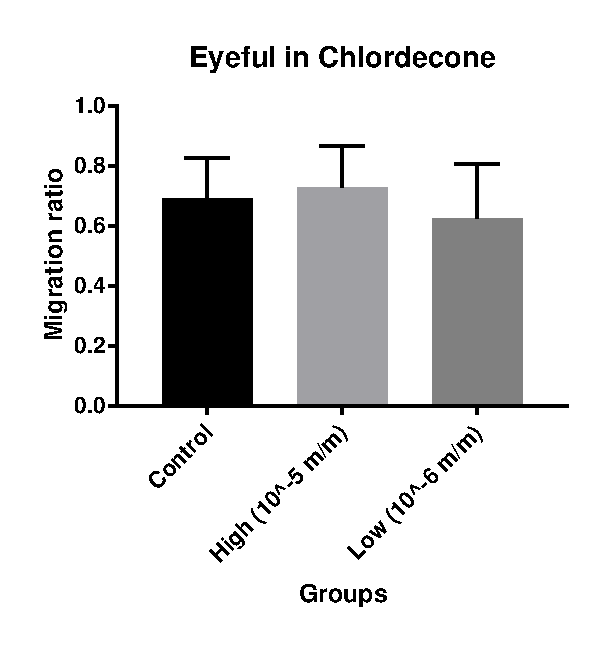
\includegraphics[width=0.6\textwidth,angle=0]{image/Data1.eps}
    \caption{The ratio of eye tumour metastases}
    \label{Eye}
\end{figure}



\subsubsection{Survival curve}
The survival curve of parent adults in different environments is shown in the figure below.
\begin{figure}[H]
    \centering
    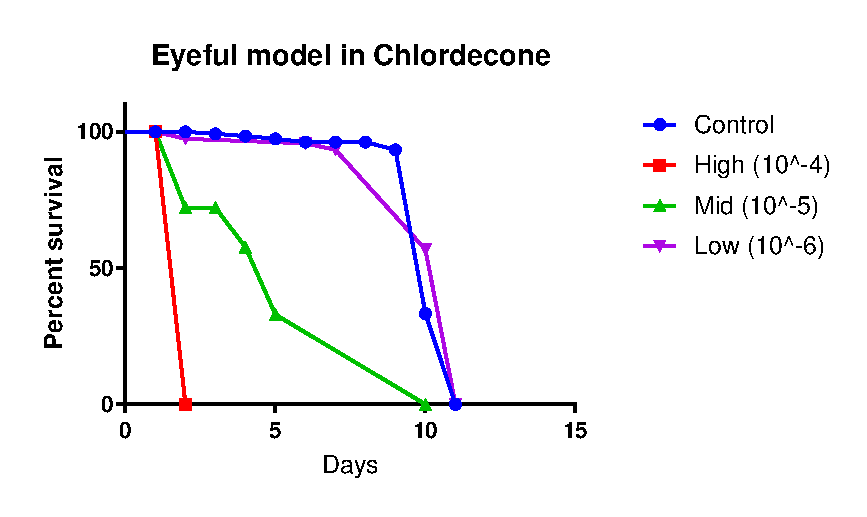
\includegraphics[width=0.7\textwidth,angle=0]{image/Data3.eps}
    \caption{Survival curve of parent adults}
    \label{D3}
\end{figure}



\subsubsection{Discussion}
Due to the small number of samples (n=12 for control group, n=11 for $10^{-5}$ group, n=8 for $10^{-6}$ group), the t-test did not give out significant results, but the figure suggests a tendency of hormesis. Low concentration seems to repress the tumour metastases, while 10 folds higher concentration leads to slightly more tumour metastases.

The fact that no significant changes can be found in tumour metastases may result from the difference in the survival rate of parent adults, which is confirmed by the survival curve and the statistical analysis (**** significance). Low F1 survival rate indicates a low survival rate of the F1, which can balance the influence of Chlordecone on tumour metastases.

\newpage
\section{Report 05: POPs treatment of the $Ras^{v12/Ig}$ model (Toxaphene)}

\subsection*{2021-05-13}

\subsection{Introduction}

With the $Eyeful$ model built in last experiment, we are now able to use different kind of POPs to treat the model flies and collect relevant data about the impact of POPs on \textbf{tumor migration}.

Other phenotypes, such as the \textbf{adult survival rate}, \textbf{reproductive capacity} and \textbf{body weight} will also be measured, if possible. These data can be used to study the overall effects of POPs, and they can provide clues about the factors behind tumor migration.

\subsection{Experiment Design}

\subsubsection{POPs gradients}
The setting of the POPs gradients used in the experiments is of much importance for their implementation.
For the convenience of calculation and dilution, we choose \textbf{Mass fraction} ($m_{POPs}/m_{fly food}$) as the unit of concentration.
According to previous literature and the real situation of the POPs pollution, we choose several POPs, which are listed in the table below. Considering that solvent should not pose much impact to our model, we choose \textbf{Dimethyl Sulfoxide (DMSO)} as the solvent for the hydrophobic POPs (in this experiment, Chlordecone). The POPs is dissolved in DMSO, and the added directly in to fly food.
As to the concentration of POPs, we started at $10^{-4}$ and dilute 10x to $10^{-6}$ to make a gradient of three concentrations, according to previous report of the POPs pollution.


\subsubsection{Crossing scheme}
The $Ras^{v12/Ig}$ model consists of two lines:
\begin{enumerate}
    \item w;$Igl^4$ FRT40A UAS-$RAS^{v12}$/CyO;Sb/TM6B Tb
    \item yw ey-Flp; tub-Gal80 FRT40A; act>y+>Gal4 UAS-GFP
\end{enumerate}
The Crossing scheme is shown below.
\begin{enumerate}
    \item \female w;$Igl^4$ FRT40A UAS-$RAS^{v12}$/CyO;Sb/TM6B Tb $\times$ yw ey-Flp; tub-Gal80 FRT40A; act>y+>Gal4 UAS-$GFP$ \male
    \item \female yw ey-Flp; tub-Gal80 FRT40A; act>y+>Gal4 UAS-GFP $\times$ w;$Igl^4$ FRT40A UAS-$RAS^{v12}$/CyO;Sb/TM6B Tb \male
\end{enumerate}

\subsubsection{Measurements}
After the crossing is done, we did several measurements everyday at the same time.

\begin{enumerate}
    \item Number of adults alive in the tube (optional) 
    \item Number of egg laid (optional)
    \item Number of adults with \textbf{tumor migration}
\end{enumerate}
After each day, transfer the adults to a new tube.

\subsection{Materials \& Methods}

\subsubsection{Preparation of fly food with POPs gradients}
The steps is listed below.
\begin{enumerate}
    \item Add \SI{1000}{\micro\liter} Dimethyl Sulfoxide (DMSO) to the POPs, lable as \texttt{\#stock solution}.
    \item Vortex till the POPs is completely dissolved.
    \item Calculate the concentration of the \texttt{\#stock solution}.
    \item Dilute the \texttt{\#stock solution} to fly food to make the gradients.
    \item Pour the fly food to tubes.
\end{enumerate}

\subsubsection{Crossing of the flies}

\paragraph{Virgins}
To carry out crosses cleanly, you must start with virgin females. Female flies are capable of mating as early as possible after emerging from the pupae stage and are polyandrous(capable of mating with several males). Once mated Females can retain viable sperm for several days and this will confuse the results of a subsequent controlled mating. Therefore, it is necessary to collect enough virgins before we carry out the crossing.

\paragraph{Crossing}
In the crossing, we used the tools needed for basic fly experiments mentioned in Lab Report 04.
	
Here are the steps:
	
		\begin{enumerate}
			\item Empty the stocks before collecting the virgins.
			\item Collect the virgins for several mornings, make sure the virgins have the required phenotypes.
			\item Anesthetize the flies before making the crossing to check the phenotypes. Then put the virgins with the corresponding males in a tube. Record and mark the genotype and numbers of the files.
			\item Put the crossings in \SI{25}{\celsius} with  60-65\% relative humidity. Wait for about a week for the crossings to give the F1 flies.
			\item Collect the F1 larva of the 3rd instar with the desired phenotype.
		\end{enumerate}

\subsubsection{Record of the results}
Different from the $Eyeful$ model, the $Ras^{V12}$ model can not survive to adults, and therefore dissection is needed in order to observe tumours and metastases. The eye disc, brain and ventral nerve cord are what we need from dissection.

The equipment needed for dissection is listed below.

\begin{itemize}
    \item Dissecting microscope
    \item Two pairs of sharp forceps (Dumont, no. 5)
    \item Dissection dishes
    \item Microscope slides
    \item PBST Solution
\end{itemize}

The steps of dissection is listed below, and the protocol is from Joy S Wu \& Liqun Luo.

\begin{enumerate}
    \item Collect larva of the stage of interest.
    \item Place the larvae into a dissection dish containing cold PBST.
    \item Use two forceps to tear the larva into halves.
    \item Overturn the skin of front half of the larva.
    \item Peeling the larval cuticle apart like a banana, starting at the mouth hook. 
    \item Discard the larval body. While maintaining a grip on the mouth hook, gently remove excess tissue surrounding the eye disc, brain and ventral nerve cord.
\end{enumerate}

The eye disc, brain and ventral nerve can then be observed using a Fluorescence Microscopy.

Videos that shows how dissection works can be found on \url{https://www.janelia.org/project-team/flylight/protocols}.
\subsection{Results \& Discussion}

\subsubsection{A typical result of tumour metastases in this model}
A typical result of tumour metastases from eye disc to brain is shown below. The migrated cells are labeled with GFP.
\begin{figure}[H]
    \centering
    \includegraphics[width=0.5\textwidth,angle=0]{image/VNC.png}
    \caption{A typical result of tumour metastases}
    \label{Eyef}
\end{figure}

\subsubsection{Eye tumour metastases ratio}
The ratio of tumour metastases is shown in the figure below.

\begin{figure}[H]
    \centering
    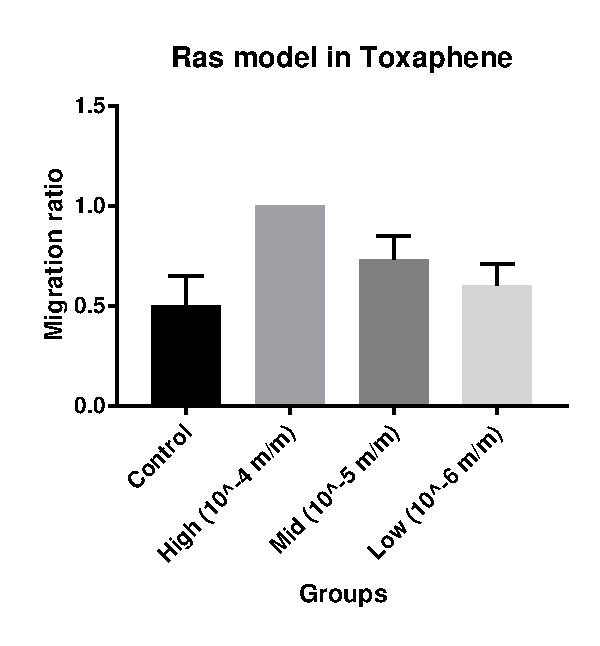
\includegraphics[width=0.6\textwidth,angle=0]{image/Data2.eps}
    \caption{The ratio of tumour metastases}
    \label{Eye}
\end{figure}

\subsubsection{Discussion}
Due to the small number of samples (n=12 for control group, n=3 for $10^{-4}$ group, n=15 for $10^{-5}$ group, n=20 for $10^{-6}$ group), the t-test did not give out significant results, but the figure suggests a tendency that higher concentration of Toxaphene is related to more tumour metastases.

We also noticed that the survival of F1 larva is affected by Toxaphene. Higher level of Toxaphene is not favourable for the survival of F1 larva, and this may cause undesirable impact on the collection of data.

\newpage
\section{Report 07: Reverse transcription qPCR}

\subsection*{2021-06-11}


\subsection{Introduction}
A real-time polymerase chain reaction (real-time PCR), also known as quantitative Polymerase Chain Reaction (qPCR), is a laboratory technique of molecular biology based on the polymerase chain reaction (PCR). It monitors the amplification of a targeted DNA molecule during the PCR (i.e., in real time), not at its end, as in conventional PCR. Real-time PCR can be used quantitatively (quantitative real-time PCR) and semi-quantitatively (i.e., above/below a certain amount of DNA molecules) (semi-quantitative real-time PCR).
		
		Real-time PCR is carried out in a thermal cycler with the capacity to illuminate each sample with a beam of light of at least one specified wavelength and detect the fluorescence emitted by the excited fluorophore. The thermal cycler is also able to rapidly heat and chill samples, thereby taking advantage of the physicochemical properties of the nucleic acids and DNA polymerase.
		
		Two common methods for the detection of PCR products in real-time PCR are (1) non-specific fluorescent dyes that intercalate with any double-stranded DNA and (2) sequence-specific DNA probes consisting of oligonucleotides that are labelled with a fluorescent reporter, which permits detection only after hybridization of the probe with its complementary sequence. In this experiment, we will use non-specific fluorescent dyes to measure the amount of PCR products.
		
		A DNA-binding dye binds to all double-stranded (ds) DNA in PCR, increasing the fluorescence quantum yield of the dye. An increase in DNA product during PCR therefore leads to an increase in fluorescence intensity measured at each cycle. However, dsDNA dyes such as SYBR Green will bind to all dsDNA PCR products, including nonspecific PCR products (such as Primer dimer). This can potentially interfere with, or prevent, accurate monitoring of the intended target sequence.
		
		In real-time PCR with dsDNA dyes the reaction is prepared as usual, with the addition of fluorescent dsDNA dye. Then the reaction is run in a real-time PCR instrument, and after each cycle, the intensity of fluorescence is measured with a detector; the dye only fluoresces when bound to the dsDNA (i.e., the PCR product). This method has the advantage of only needing a pair of primers to carry out the amplification, which keeps costs down; multiple target sequences can be monitored in a tube by using different types of dyes.
		
		The amount of an expressed gene in a cell can be measured by the number of copies of an RNA transcript of that gene present in a sample. In order to robustly detect and quantify gene expression from small amounts of RNA, amplification of the gene transcript is necessary. The polymerase chain reaction (PCR) is a common method for amplifying DNA; for RNA-based PCR the RNA sample is first reverse-transcribed to complementary DNA (cDNA) with reverse transcriptase.
		
		Estimation errors arising from variations in the quantification method can be the result of DNA integrity, enzyme efficiency and many other factors. For this reason a number of standardization systems (often called normalization methods) have been developed. Some have been developed for quantifying total gene expression, but the most common are aimed at quantifying the specific gene being studied in relation to another gene called a normalizing gene, which is selected for its almost constant level of expression. These genes are often selected from housekeeping genes as their functions related to basic cellular survival normally imply constitutive gene expression. \cite{vandesompele2002accurate} This enables researchers to report a ratio for the expression of the genes of interest divided by the expression of the selected normalizer, thereby allowing comparison of the former without actually knowing its absolute level of expression. The most commonly used normalizing genes are those that code for the following molecules: tubulin, glyceraldehyde-3-phosphate dehydrogenase, albumin, cyclophilin, and ribosomal RNAs. \cite{wiki2018qpcr}


\subsection{Experiment Design}
We picked several genes in the pathways that previous studies show to be related to tumor metastases. The primers used in the qPCR is listed below, for detailed primer sequence, please contact the authors of this report.

\begin{enumerate}
    \item Rho1: Negative Regulators of Wnt-TCF Signaling Pathway
    \item Toll6: TOLL RECEPTORS
    \item sna: A transcription factor that contributes to embryonic mesoderm development, epithelial to mesenchymal transition and asymmetric cell division.
    \item Ben: Positive Regulators of TNF$\alpha$-Eiger Signaling Pathway
    \item Wnd: axonal injury signaling
    \item Src42A: Negative/Positive Regulators of EGFR Signaling Pathway and Positive Regulators of Sevenless Signaling Pathway
    \item PucA
    \item Rac1: Pvr Signaling Pathway Core Components
    \item Diap1: Death-associated inhibitor of apoptosis 1
    \item RP49: reference gene
\end{enumerate}

The eyeful model treated in Chlordecone is used as the sample (with the 0 concentration of Chlordecone in DMSO added to eyeful fly food as a control), and w1118 is used as another control group.
		
The annealing temperature is set to \SI{60}{\celsius}, which is compatible with our primers.

\subsection{Materials \& Methods}
    \subsection{Materials}
			In this experiment, we used the \texttt{Agilent Mx3000P QPCR System} for the qPCR reactions.
			
			The reagents we used are listed below.
			
			\begin{enumerate}
				\item Eastep\textregistered Super Total RNA Extraction Kit
					\subitem Nuclease-Free Water
					\subitem DNAse I (lyophilized)
					\subitem 1-Thioglycerol
					\subitem 10XDNA I Buffer, Bulk
					\subitem RNA Wash Solution (RWA)
					\subitem RNA Dilution Buffer (RDB)
					\subitem Lysis Buffer (LBA)
				\item TransScript\textregistered All-in-One First-Strand cDNA Synthesis SuperMix for qPCR (+gDNA Removal)
					\subitem TransScript\textregistered 5x All-in-One SuperMix for qPCR
					%\subitem TransScript$^{\tiny{\textregistered}}$ 5x All-in-One No-RT Control SuperMix for qPCR
					\subitem gDNA Remover
					\subitem RNase-free Water 
				\item TransStart\textregistered Top Green qPCR SuperMix
			\end{enumerate}
    \subsection{Methods}
		
		The first part of this experiment is reverse transcription of mRNA. Steps are listed below.
		
		\begin{enumerate}
			\item Freeze the fruit flies in \SI{-80}{\celsius} refrigerator for 20 mins.
			\item Homogenate the fruit files in EP tubes together with RNA lysis buffer.
			\item Add RNA Dilution Buffer to EP tubes, mix the buffer with the solution in the EP tubes and then centrifuge at maximum speed for 5 minutes.
			\item Add 0.5 times of the original volume of ethanol to the EP tubes, vortex.
			\item Transfer the mixture to the Spin Column, centrifuge at 12000-14000xg for 1 min, then dispose the aqueous phase.
			\item Add \SI{600}{\uL} RNA wash solution, centrifuge at 12000-14000xg for 45 sec, then dispose the aqueous phase.
			\item Add \SI{50}{\uL} DNAse I and incubate for 15 min.
			\item Add \SI{600}{\uL} RNA wash solution, centrifuge at 12000-14000xg for 45 sec, then dispose the aqueous phase.
			\item Centrifuge at 12000-14000xg for 2 min, keep the aqueous phase.
			\item Add \SI{100}{\uL} Nuclease-Free water, centrifuge at 12000-14000xg for 2 min, keep the aqueous phase.
			\item Prepare the EP Tubes and mark the genotype of the files of each tube.
			\item Add \SI{4}{\uL} TransScript$^{\tiny{\textregistered}}$ 5x All-in-One SuperMix for qPCR, \SI{1}{\uL} gDNA Remover, \SI{5}{\uL} cell lysis solution and \SI{10}{\uL} RNase-free Water to each tube.
			\item Put the Tubes into the rt machine and run the reverse transcription program.
		\end{enumerate}
	
		The second part of this experiment is the quantitative PCR. Steps are listed below.
		
		\begin{enumerate}
			\item Prepare the 8-Strip PCR Tubes and mark the experiment group of each tube. Note that do not make marks on the top of PCR Tubes.
			\item Add \SI{10}{\uL} SYBR Green Master Mix to each PCR tube.
			\item Add \SI{1}{\uL} template, \SI{0.4}{\uL} forward primer and \SI{0.4}{\uL} reverse primer to each PCR tube.
			\item Add \SI{8.2}{\uL} RNase-free Water to each PCR tube.
			\item Put the 8-Strip PCR Tubes into \texttt{Agilent Mx3000P QPCR System}, set the annealing temperature to \SI{60}{\celsius} and run the qPCR program.
			\item Dispose the 8-Strip PCR Tubes following the lab regulations.
		\end{enumerate}


\subsection{Results \& Discussion}

The results of the qPCR is summarized in the figure below.

\begin{figure}[H]
    \centering
    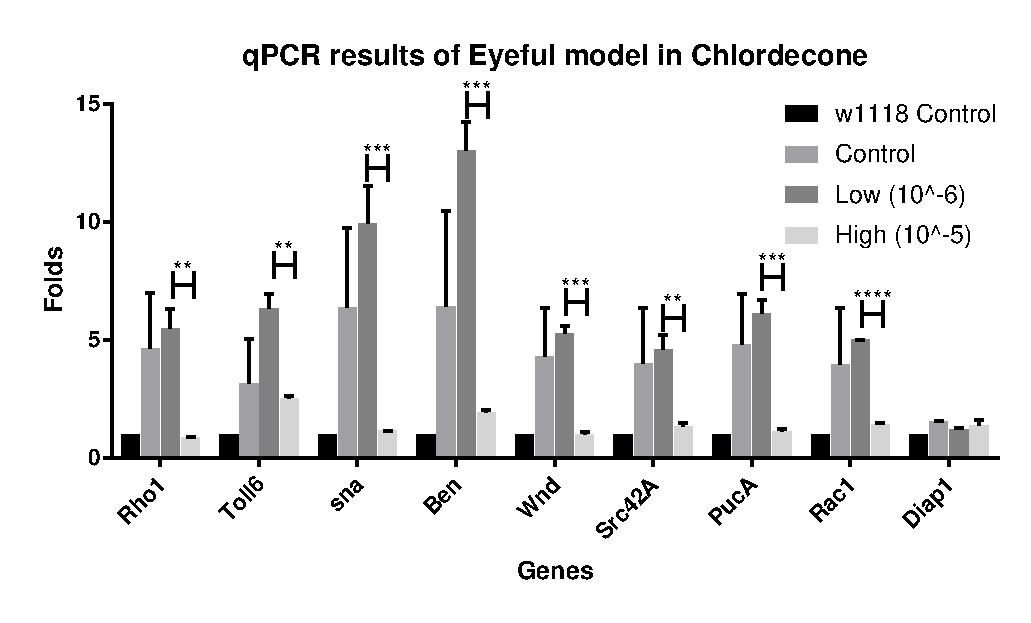
\includegraphics[width=1\textwidth,angle=0]{image/Data4.eps}
    \caption{qPCR results}
    \label{qpcr}
\end{figure}

From the results, we can find that except the Diap1, other 8 genes showed significantly difference (more than ** significance in t test) in mRNA level when treated with different concentration of Chlordecone. However, the transcription level of these genes are not in proportion to the Chlordecone concentration, that is, the relation between Chlordecone concentration and transcription level of these genes is not linear. This indicates a possible hormesis phenomenon of these genes when the fly is treated with POPs like Chlordecone. 

The results of our qPCR is consistent with the result of our previous observation of the tumor metastases in the eyeful model when treated with Chlordecone. Many of the selected genes in our qPCR showed higher transcription in low Chlordecone concentration environment, while in high Chlordecone concentration environment, the transcription level is a little lower, and the tumor metastases ratio of the flies follows the same trend. This may suggest the connection between POPs treatment, suspicious relevant pathways and the phenotype.

\newpage
\section*{Acknowledgements}
Throughout the course in this semester I have received a great deal of support and assistance.
I would first like to thank my supervisor, Associate Professor Wenzhe Li, whose expertise was invaluable in formulating the research questions and methodology. Your insightful feedback pushed me to sharpen my thinking and brought my work to a higher level.

I would like to acknowledge my classmates from School of life science for their wonderful collaboration and assistance in the experiments. I would particularly like to single out my team members in our SITP Project: Chen Keyinglu, He Fenglian and Yang Jiani, I want to thank you for your patient support in this course and the project.

I would also like to thank my tutor, Professor Lei Xue for his valuable guidance throughout my studies. You provided me with the tools that I needed to choose the right direction.

\bibliography{references}

\end{document}